\documentclass[11pt,cmyk,a4paper,colorscheme=green,TUBStitlepage=picture]{tubsartcl}

\usepackage[noxcolor]{beamerarticle}
\usepackage{tubscolors}
\usepackage{nexus}
\usepackage{amssymb}

\usepackage[ngerman]{babel}

% \usetheme{tubs}
% \usepackage{ifwlogo}
% \usepackage[blue]{TU-CDcolors}
% \usepackage{uarial}

% \usepackage[T1]{fontenc}
\usepackage[utf8x]{inputenc}

\date{\today}
\subject{Anleitung und Dokumentation}
\title{Design oder nicht sein?}
\subtitle{Das Corporate Design in  LaTeX}
\author{Martin Bäker  Enrico Jörns}
\titlegraphic{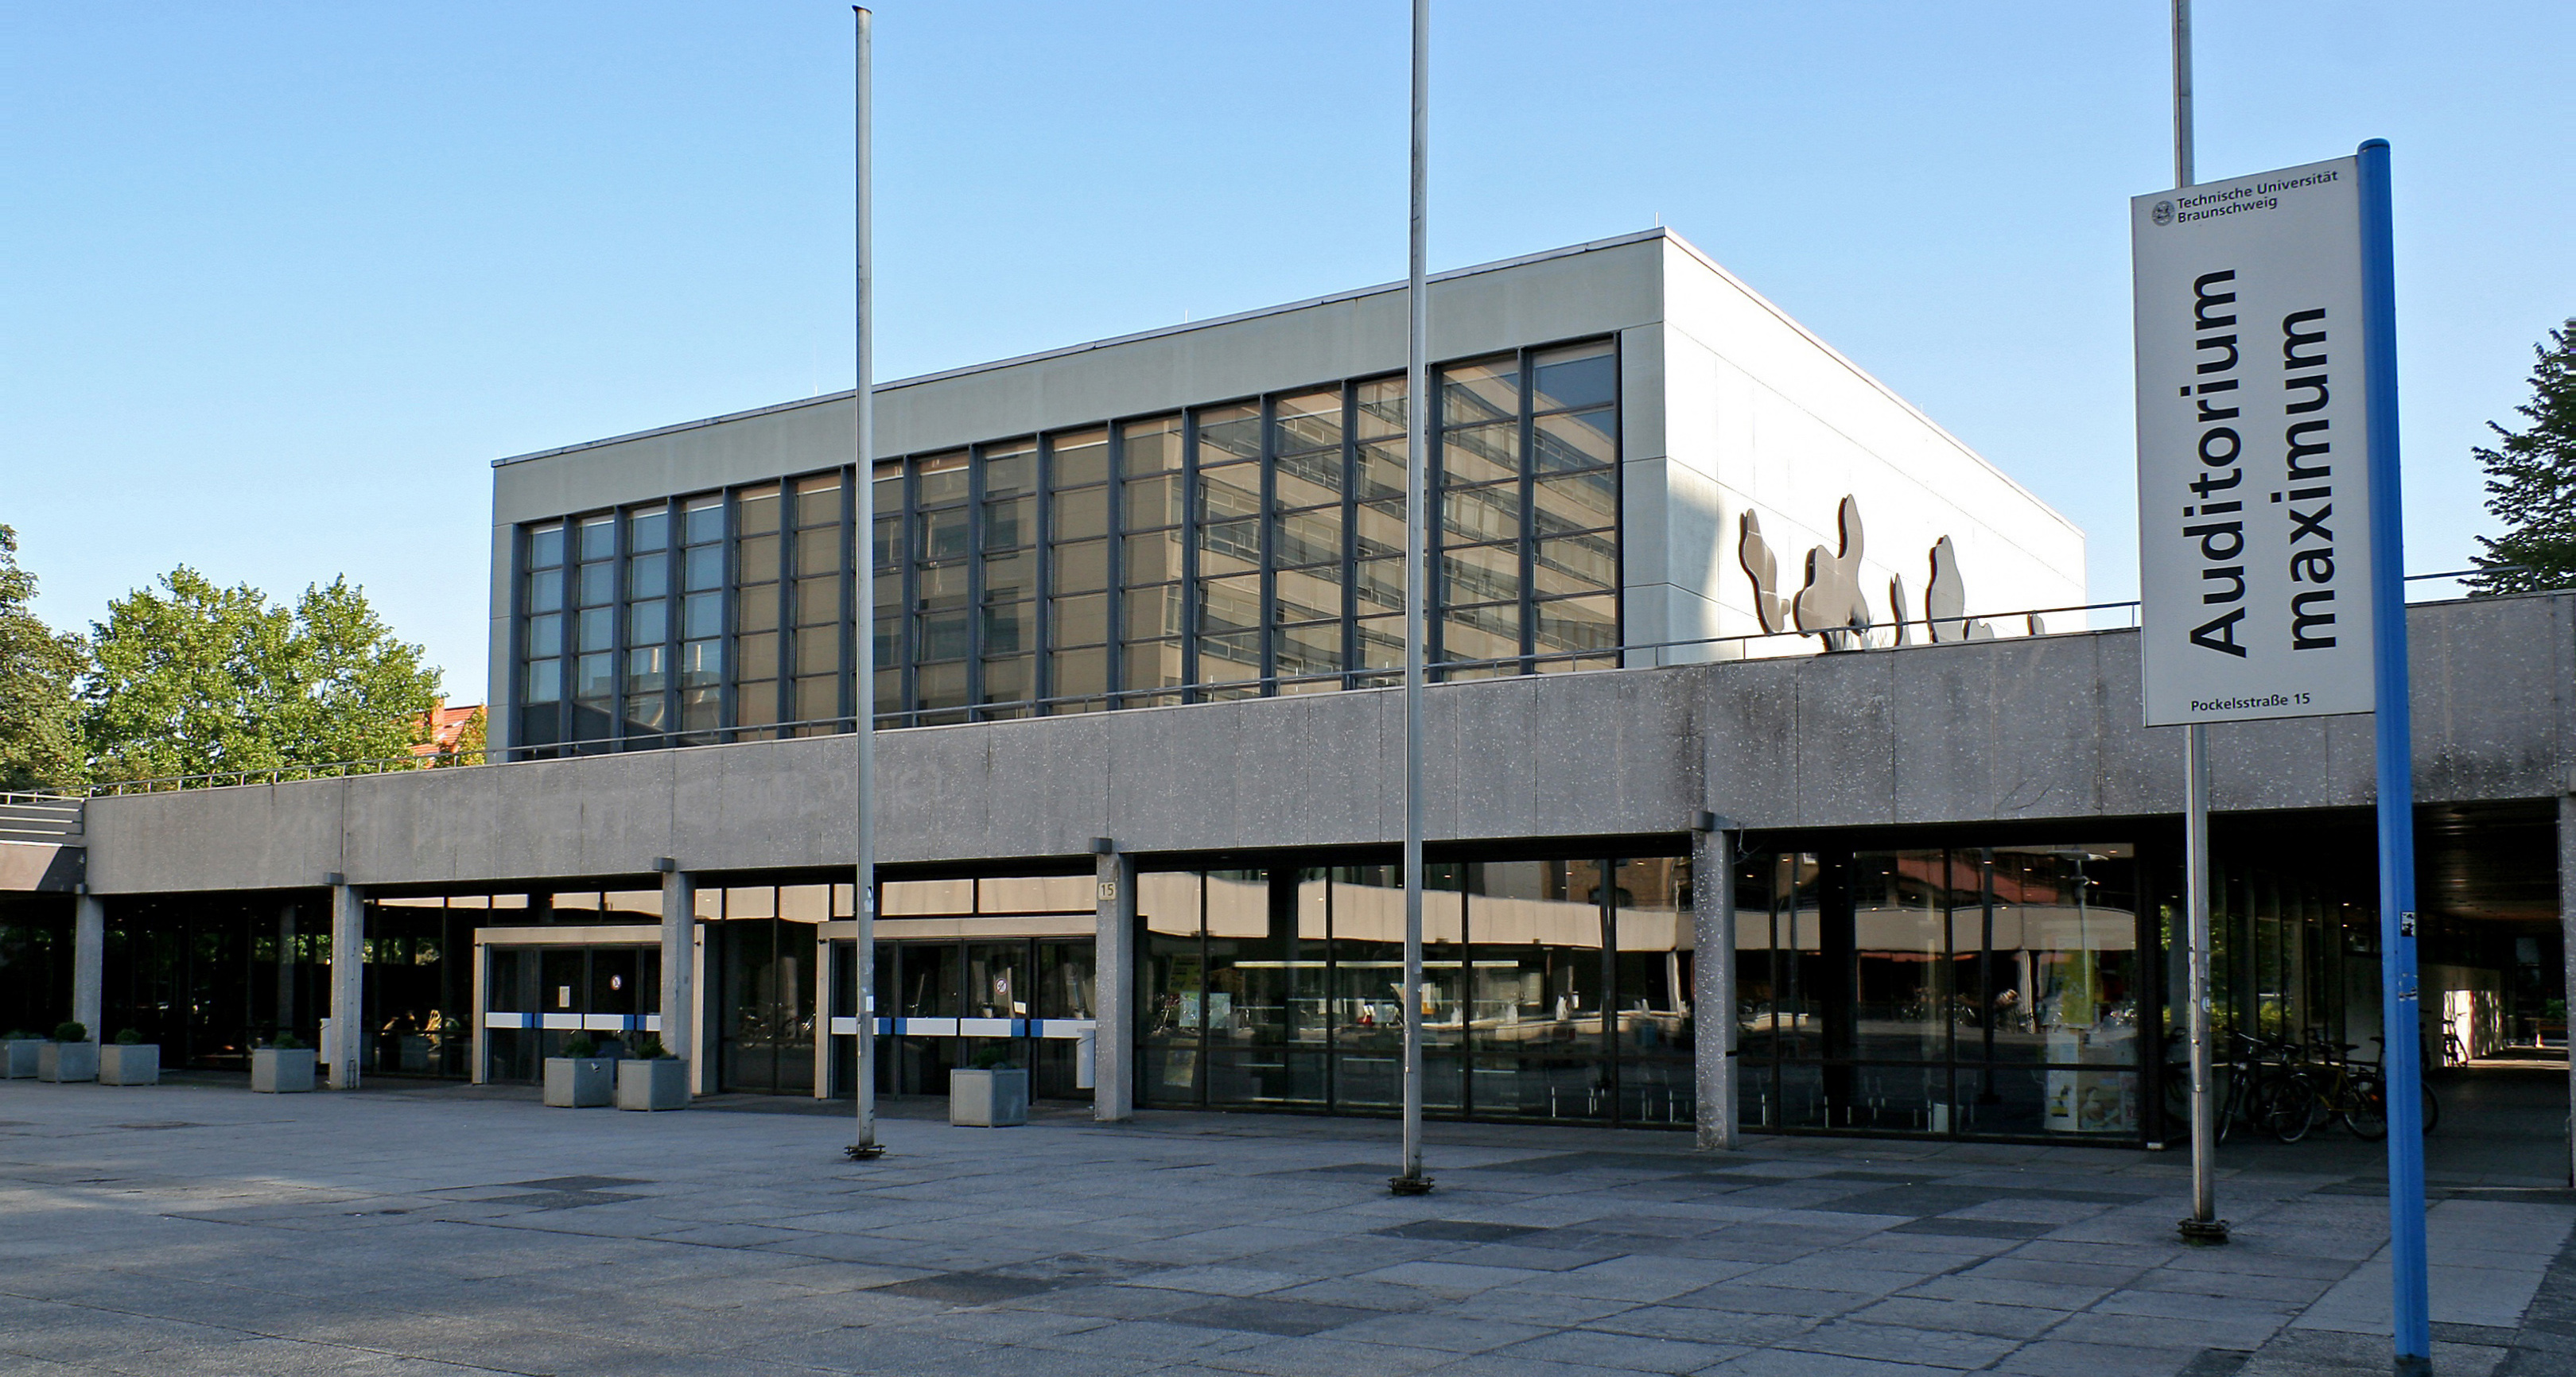
\includegraphics[width=\titlegraphicswidth]{titlepicture}}
% \logo{
\includegraphics[height=\logoheight]{institut.jpg}}
\logo{Institut für Unkreativität\\und Schreibschwäche}
\institute{asdf}

\begin{document}

\maketitle

\begin{frame}[plain]
\titlepage
\end{frame}

\begin{frame}{Inhalt}
\tableofcontents
\end{frame}

\section{Anfang}

\subsection{Anfang 1}

\begin{frame}{Itemize-Test}
  \begin{itemize}
    \item Lorem ipsum dolor sit amet, consetetur sadipscing elitr, sed diam
      nonumy eirmod tempor invidunt ut labore et dolore magna aliquyam
    \item At vero eos et accusam et justo duo dolores et ea rebum.
      \begin{itemize}
        \item Stet clita kasd gubergren, no sea takimata sanctus est Lorem ipsum
          dolor sit amet!
          \begin{itemize}
            \item Nam eget dui.
            \item Maecenas tempus, tellus eget condimentum rhoncus, sem quam
              semper libero, sit amet adipiscing sem neque sed ipsum.
          \end{itemize}
        \item Duis leo
      \end{itemize}
    \item Aliquam lorem ante, dapibus in, viverra quis, feugiat a, tellus. 
  \end{itemize}
\end{frame}

\subsection{Anfang 2}

\begin{frame}{Mathe-Test}
  Gaußsche Summenformel:
  \[1 + 2 + 3 + 4 + \ldots + n = \sum_{k=1}^n k = \frac{n(n+1)}{2}\]
  Faltung:
  \[(f*g)(\xi) := \int_{\mathbb{R}^n} f(y)g(\xi-y)\mathrm{d}y\]
\end{frame}

\section{Ende}

\begin{frame}{Farbtest}
  {\color{tuRed}
  Dies ist ein Text in tuRed.}

  {\color{tuSecondaryDark80}
  Dies ist ein Text in tuSecondaryDark80.}

  {\color{tuSecondaryLight}
  Dies ist ein Text in tuSecondaryLight.}

  \begin{block}{Diest ist ein Block}
    Lorem ipsum dolor sit amet, consetetur sadipscing elitr, sed diam
    nonumy eirmod tempor invidunt ut labore et dolore magna aliquyam
  \end{block}
  
  \begin{exampleblock}{Diest ist ein Example-Block}
    Lorem ipsum dolor sit amet, consetetur sadipscing elitr, sed diam
    nonumy eirmod tempor invidunt ut labore et dolore magna aliquyam
  \end{exampleblock}

  \begin{alertblock}{Diest ist ein Alert-Block}
    Lorem ipsum dolor sit amet, consetetur sadipscing elitr, sed diam
    nonumy eirmod tempor invidunt ut labore et dolore magna aliquyam
  \end{alertblock}
\end{frame}

\begin{frame}{Hier steht der Titel der Folie}
Wir beginnen mit einer Aufzählung
\begin{itemize}
\item Aufzählzeichen sind Quadrate
\begin{itemize}
\item Unterpunkte bekommen auch Quadrate
\item Wem das nicht gefällt, der kann es im beamerinnertheme ändern,
  kriegt aber dann Ärger mit der Designpolizei
\end{itemize}
\end{itemize}

\end{frame}


% \begin{highlightframe}{Wichtig}
% Diese Folie ist wichtig!
% \end{highlightframe}



\end{document}
